% !TEX encoding = UTF-8
% !TEX TS-program = pdflatex
% !TEX root = ../Tesi.tex
% !TEX spellcheck = en-EN

% %************************************************
% \chapter{Sinter Segregator}
% \label{cap:sintersegregator}
% %************************************************

\section{Design}
\label{sec:design}

\begin{figure}[!htb]
\centering
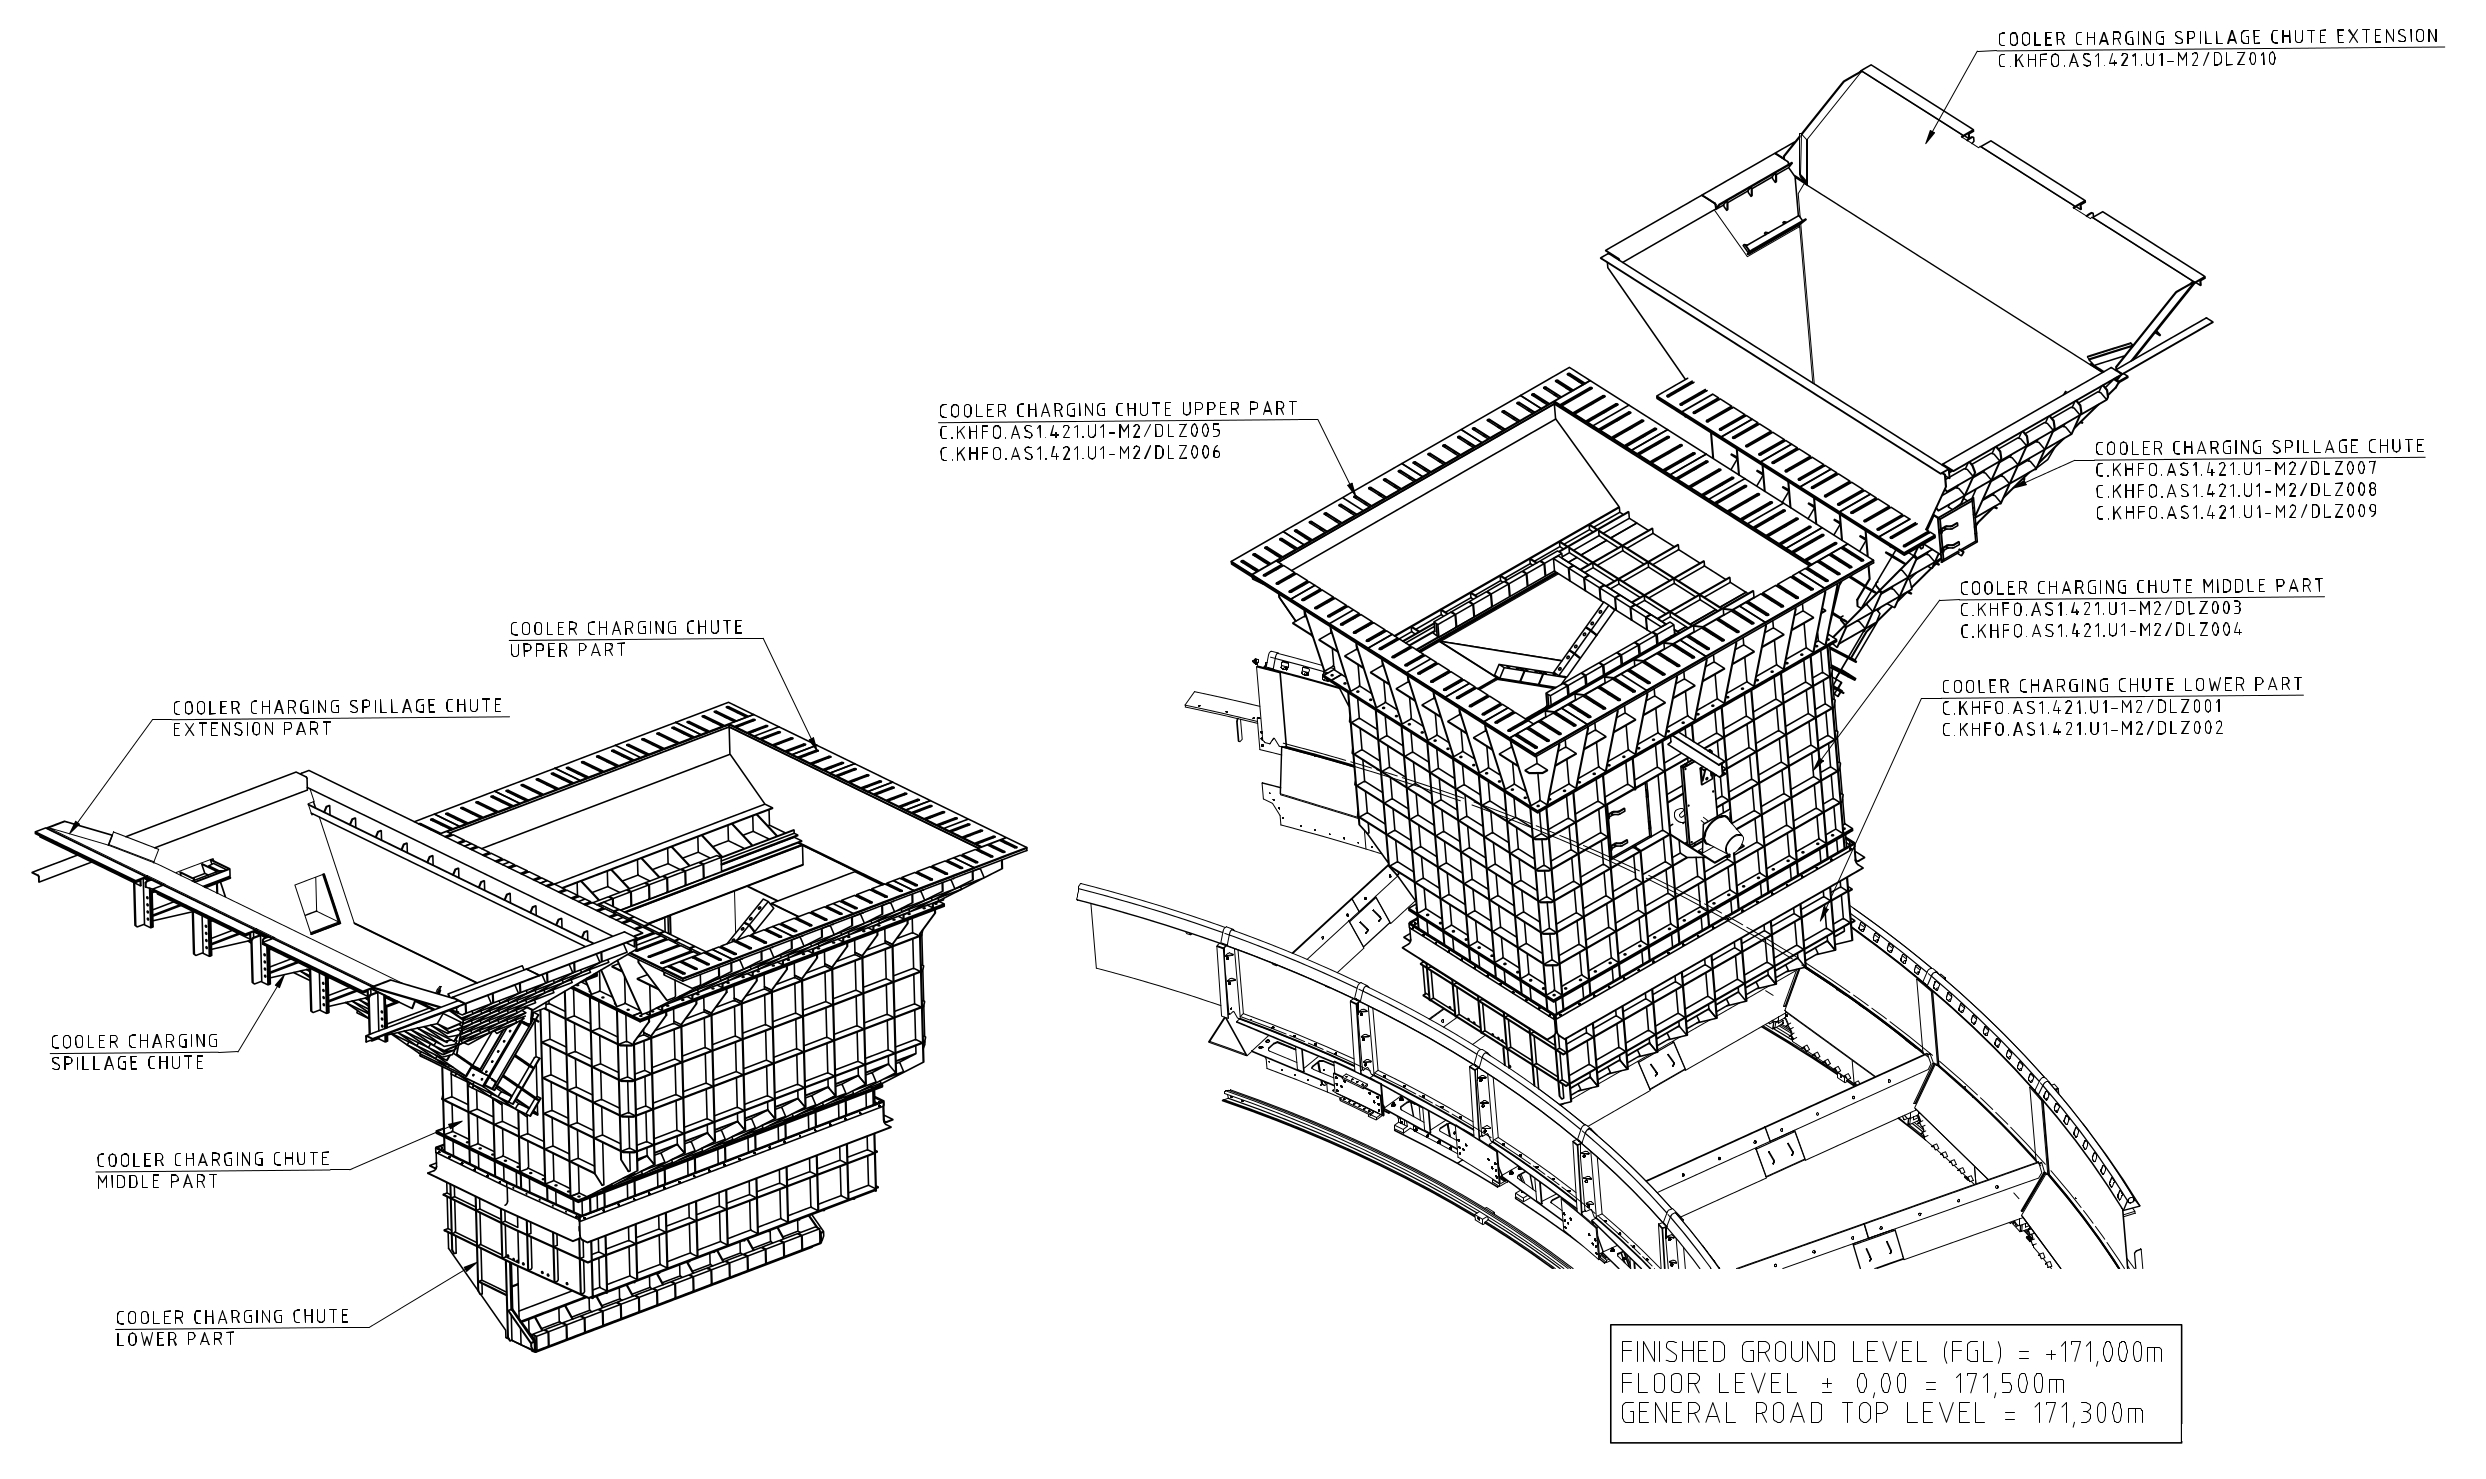
\includegraphics[width=.80\columnwidth]{images/057sinterChuteOrtoLayout}
\caption[Sinter chute orto layout]{Sinter chute orto layout.}
\label{fig:057sinterChuteOrtoLayout}
\end{figure}

The method presented in the article \textit{Characterization of Particle Based Simulation Parameters
by means of Artificial Neural Networks} allowed to collect data
regarding the contact law parameters
for the \textit{Discrete Element Method (DEM)} simulations involving sinterized
ore.
We took the average value for each of the $DEM$ parameter and we used them 
in the industrial scale $DEM$ simulation, with the same software, 
of an iron ore sintering process, see Fig. \ref{fig:057sinterChuteOrtoLayout}.
Especially, we examined the behaviour of these particles in the sinter chute
cooler.

\begin{figure}[!htb]
\centering
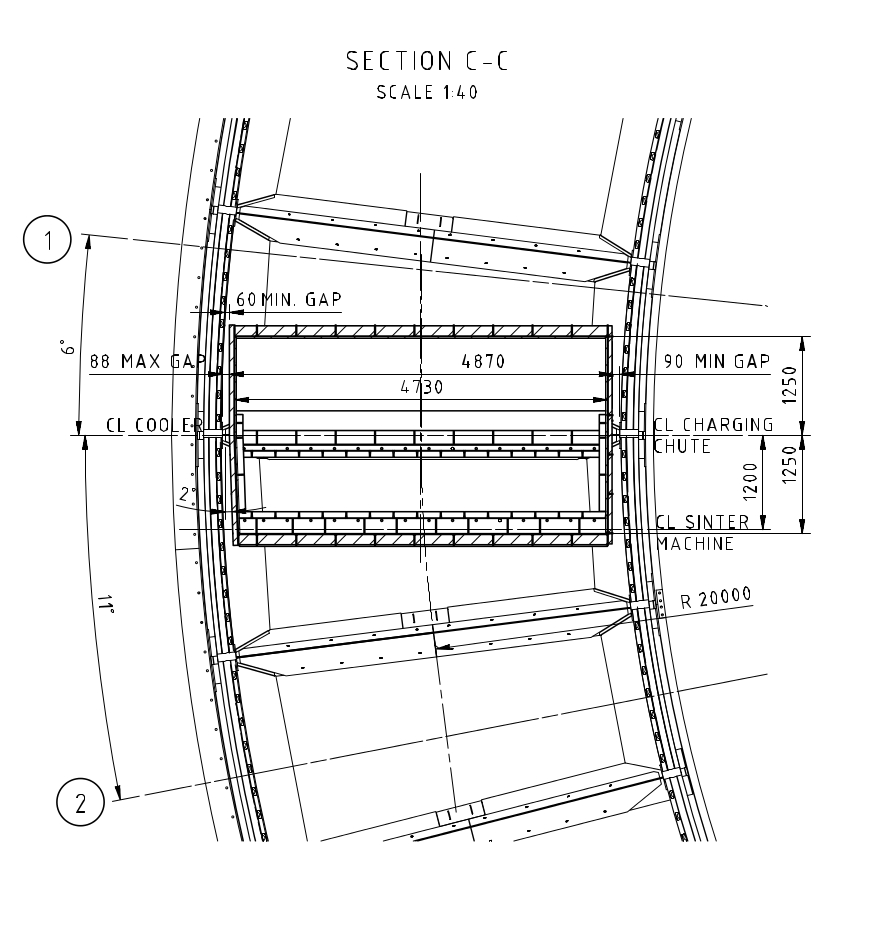
\includegraphics[width=.80\columnwidth]{images/056sinterChuteBox}
\caption[Sinter chute box]{Sinter chute box (Primetals GmbH).}
\label{fig:056sinterChuteBox}
\end{figure}

The particles moved from the top of a specifically designed chute and were 
collected by moving boxes at the bottom. These boxes were holed at the base, 
allowing cool air to lower the temperature of the sinter. 
It was critical to ascertain if the larger particles segregated, 
by moving to the bottom of the boxes (see Fig. \ref{fig:056sinterChuteBox}), while the smaller to the top,
allowing a more effective distribution of the cool air. 
Especially, the regions
highlighted in Fig. \ref{fig:055sinterChuteVerticalLayout} and
Fig. \ref{fig:067sinterchute} for the simulation were investigated.
The simulation was performed with a maximum of 500,000 particles.
For a $DEM$ simulation is a huge number, obtained with a coarse graining factor
of five, meaning that all the particles have radii five time larger than reality.
Avoiding coarse graining would have meant more than 10,000,000 particles,
infeasible for us.

\begin{figure}[!htb]
\centering
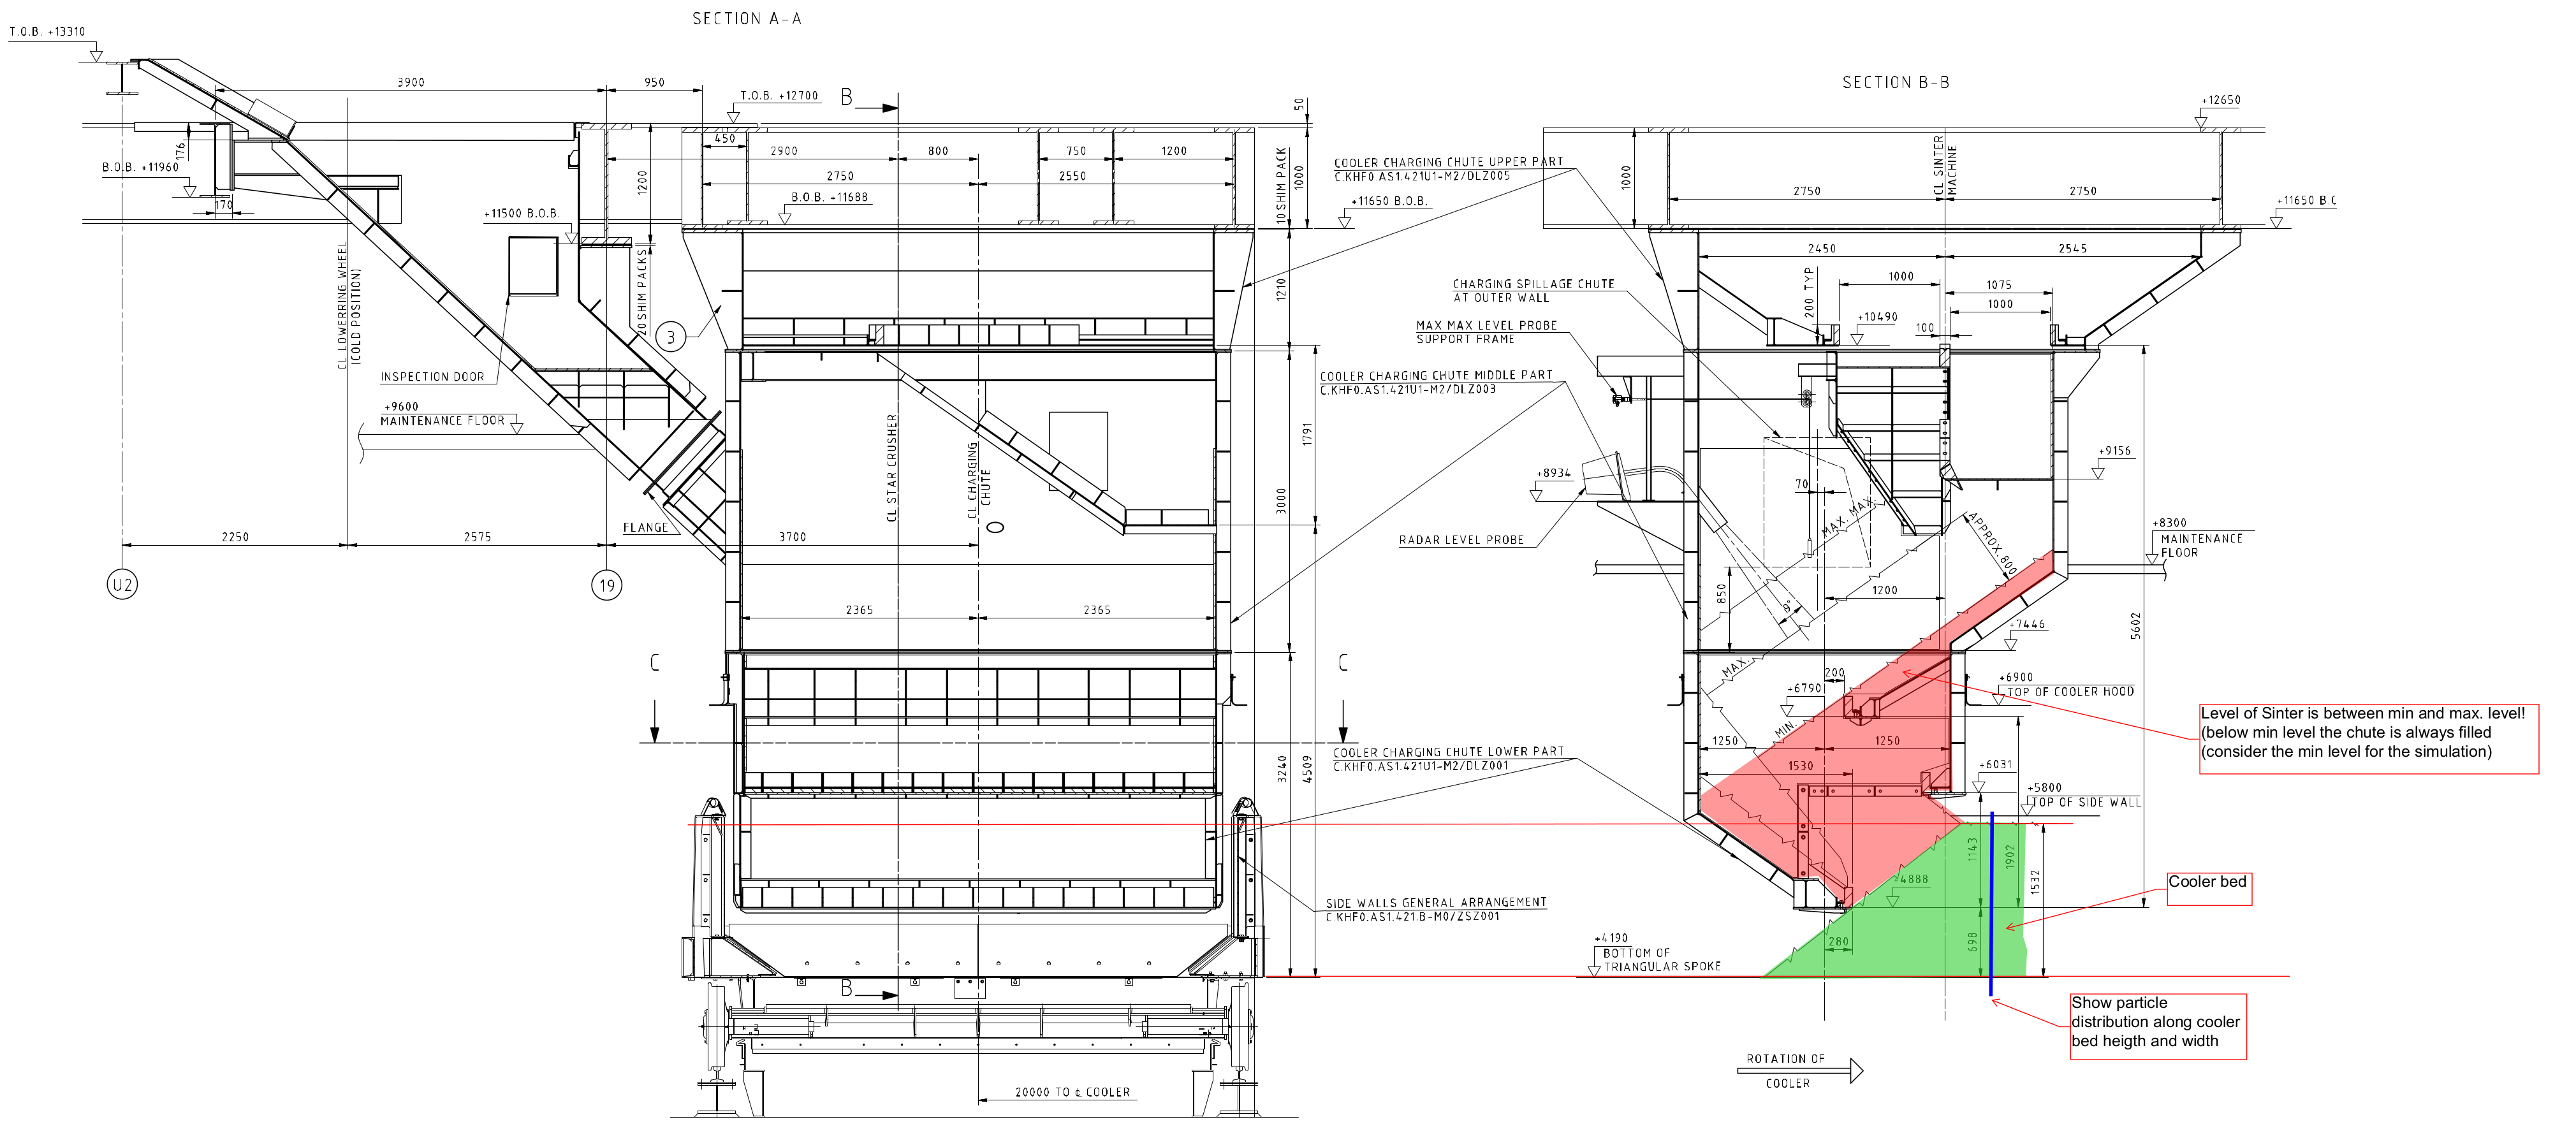
\includegraphics[width=.80\columnwidth]{055sinterChuteVerticalLayout}
\caption[Sinter chute vertical layout]{Sinter chute vertical layout.}
\label{fig:055sinterChuteVerticalLayout}
\end{figure}
\begin{figure}[!htb]
\centering
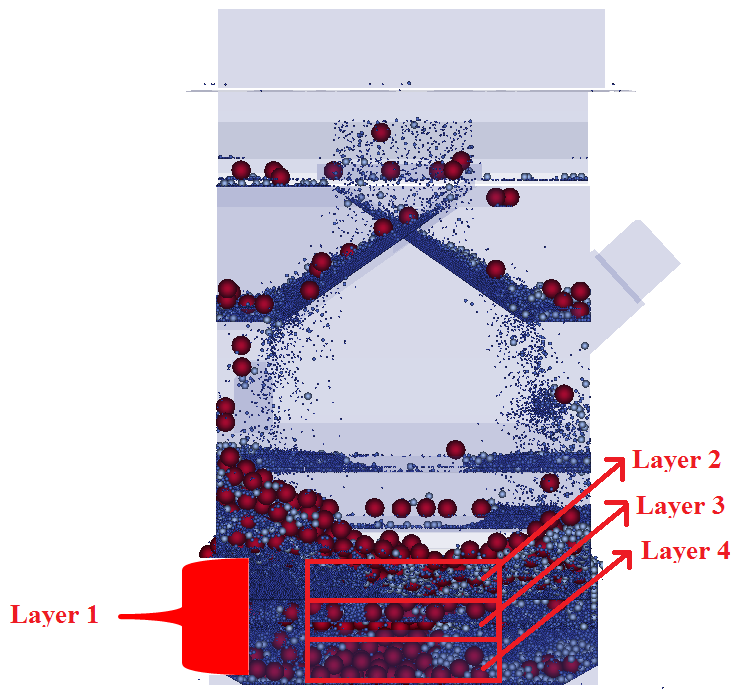
\includegraphics[width=.80\columnwidth]{images/067sinterchute}
\caption[Sinter chute simulation]{Sinter chute simulation.}
\label{fig:067sinterchute}
\end{figure}

\section{Results}
\label{sec:results}

\begin{figure}[htbp]
\centering 
    \subfloat[Frontal view. t = 150 s.]{
	  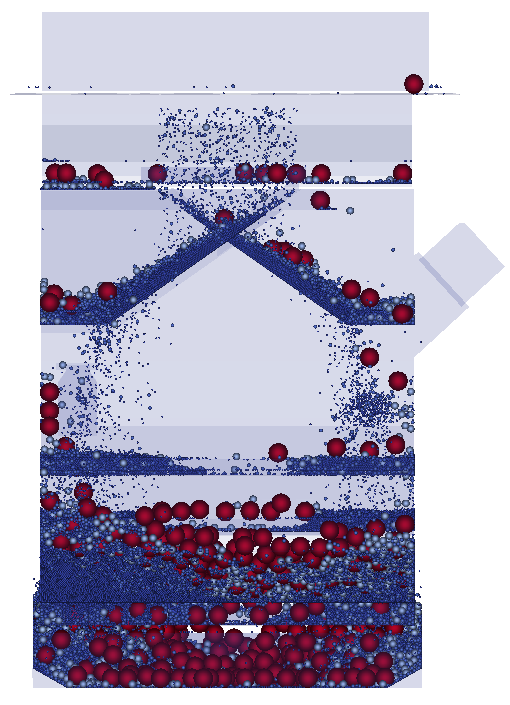
\includegraphics[width=.25\columnwidth]{images/303frontalLayout150}
	  \label{fig:303frontalLayout150}  }
 \quad
   \subfloat[Lateral view. t = 150 s.]{
	  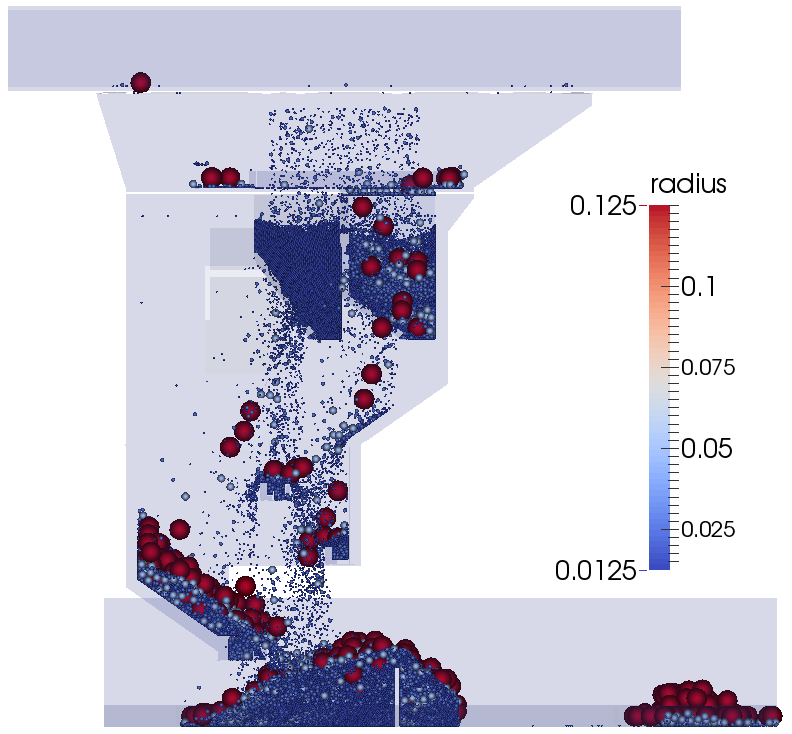
\includegraphics[width=.37\columnwidth]{images/305lateralLayout150}
	  \label{fig:305lateralLayout150}  }
  \\
  \subfloat[Frontal view. t = 200 s.]{
	  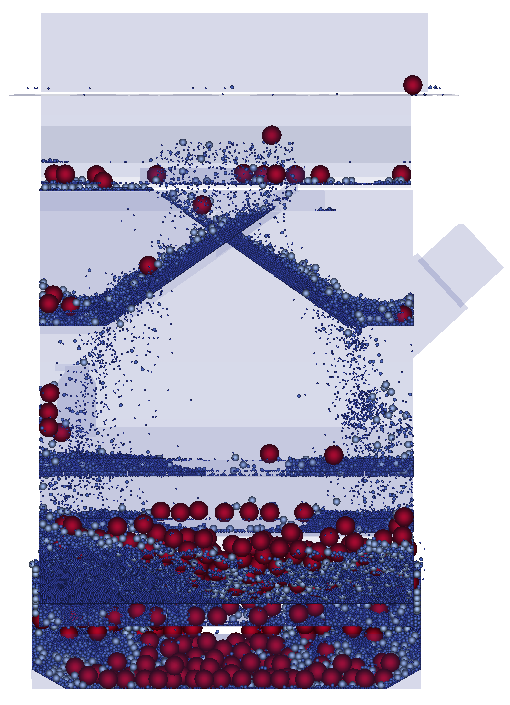
\includegraphics[width=.25\columnwidth]{images/304frontalLayout200}
	  \label{fig:304frontalLayout200}  }
  \quad 
  \subfloat[Lateral view. t = 200 s.]{
	  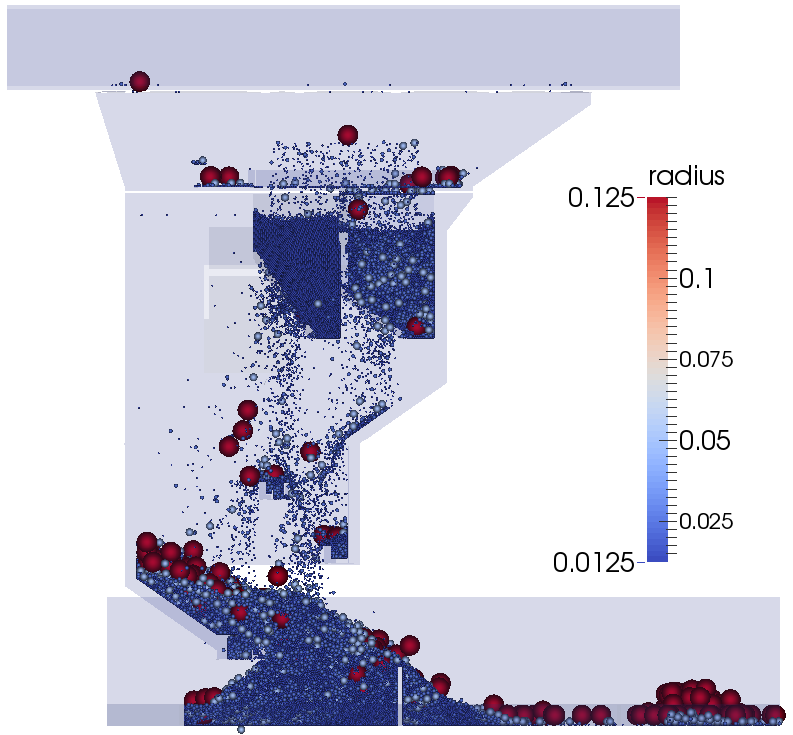
\includegraphics[width=.37\columnwidth]{images/306lateralLayout200}
	  \label{fig:306lateralLayout200}  }
  \\
  \subfloat[Frontal view. t = 250 s.]{
	  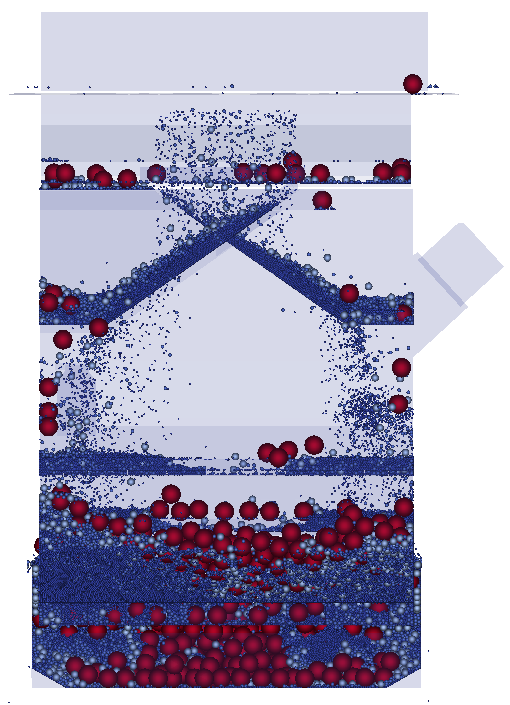
\includegraphics[width=.25\columnwidth]{images/301frontalLayout250}
	  \label{fig:301frontalLayout250}}
    \quad	  
  \subfloat[Lateral view. t = 250 s.]{
	  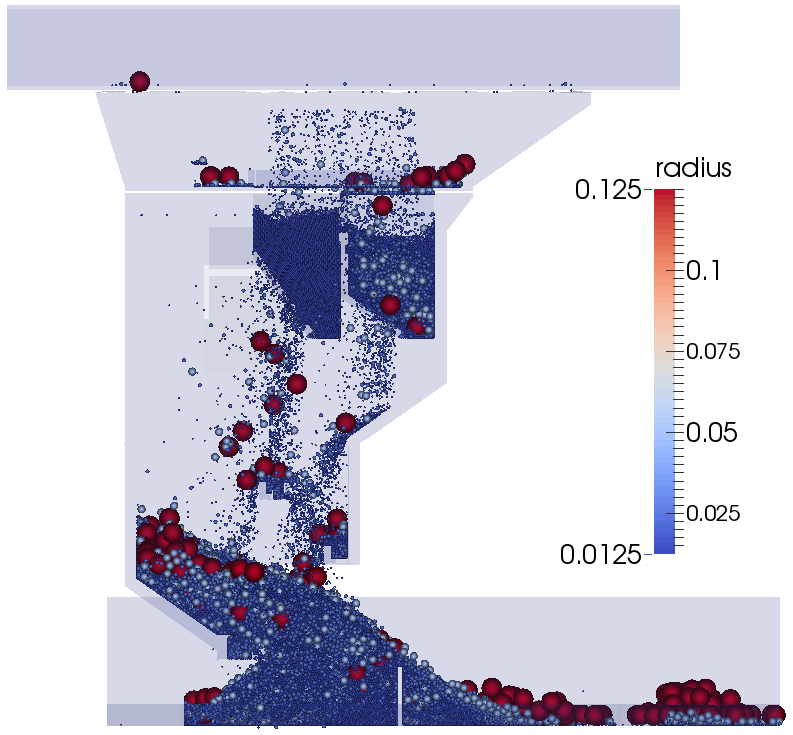
\includegraphics[width=.37\columnwidth]{images/302lateralLayout250}
	  \label{fig:302lateralLayout250}  }  
  \\
  \caption[Simulation screenshots]{Sinter chute simulation screenshots.
  Particles are tracked to ascertain the segregation behaviour.}
  \label{fig:097particlespositions}
\end{figure}
\begin{table}[htbp]
  \centering
  \caption{Particles distribution at the inlet}
    \begin{tabular}{l|cccc}
    \hline
    \#    & diameter [mm] & radius [m] & coarse grained radius [m] & \% of the
    volume
    \\
    \hline
    1     & 5     & 0.0025 & 0.0125 & 30 \\
    2     & 10    & 0.0050 & 0.0250 & 25 \\
    3     & 20    & 0.0100 & 0.0500 & 25 \\
    4     & 50    & 0.0250 & 0.1250 & 20 \\
    \hline
    \end{tabular}%
  \label{tab:radii}%
\end{table}%


Particles are inserted continuously from the top according to the particle
distribution in Table \ref{tab:radii}.
There are two main phases:
\begin{itemize}
  \item{Initial filling: during this phase many small particles deposited inside
  the chute.}
  \item{Moving bottom box: also in this phase particles were
continuously inserted from the top. After the filling was completed, the
scraper was moved and all the particles beyond a defined surface were
deleted. Inside the sinter, all the places that small particles could
occupy already were. At this point the bottom box was filled again, but
with a more realistic size distribution, and it reached steady state 
(few screenshots in Fig. \ref{fig:097particlespositions}).}
\end{itemize}
As expected, when the steady state was reached, the particles actually
segregated, as it was intended to demonstrate.
We divided the first of the boxes
filled by the chute in three (equally high) layers, from 6 on top to 8 
on bottom, see Fig. \ref{fig:056sinterChuteBox}. 
The volume over these layers was not considered, because it was continuously 
supplied of particles from the chute.
In fact, there were more particles with larger radii, from 25 to 125 mm, in the
bottom layers.
Instead, the smallest particles, radius = 12.5 mm, were rather on the top layer. 
In Fig. \ref{fig:066sinterbarplot} the
percentage of the total volume of the particles available in each layer at steady-state, 
grouped by radius, is shown. 
We could clearly see how the larger particles disposed mostly 
in the bottom layer, validating the realized design.

\begin{figure}[htbp]
\centering 
  \subfloat[Ratio over the volume occupied by the particles of each radius.]
  {
	  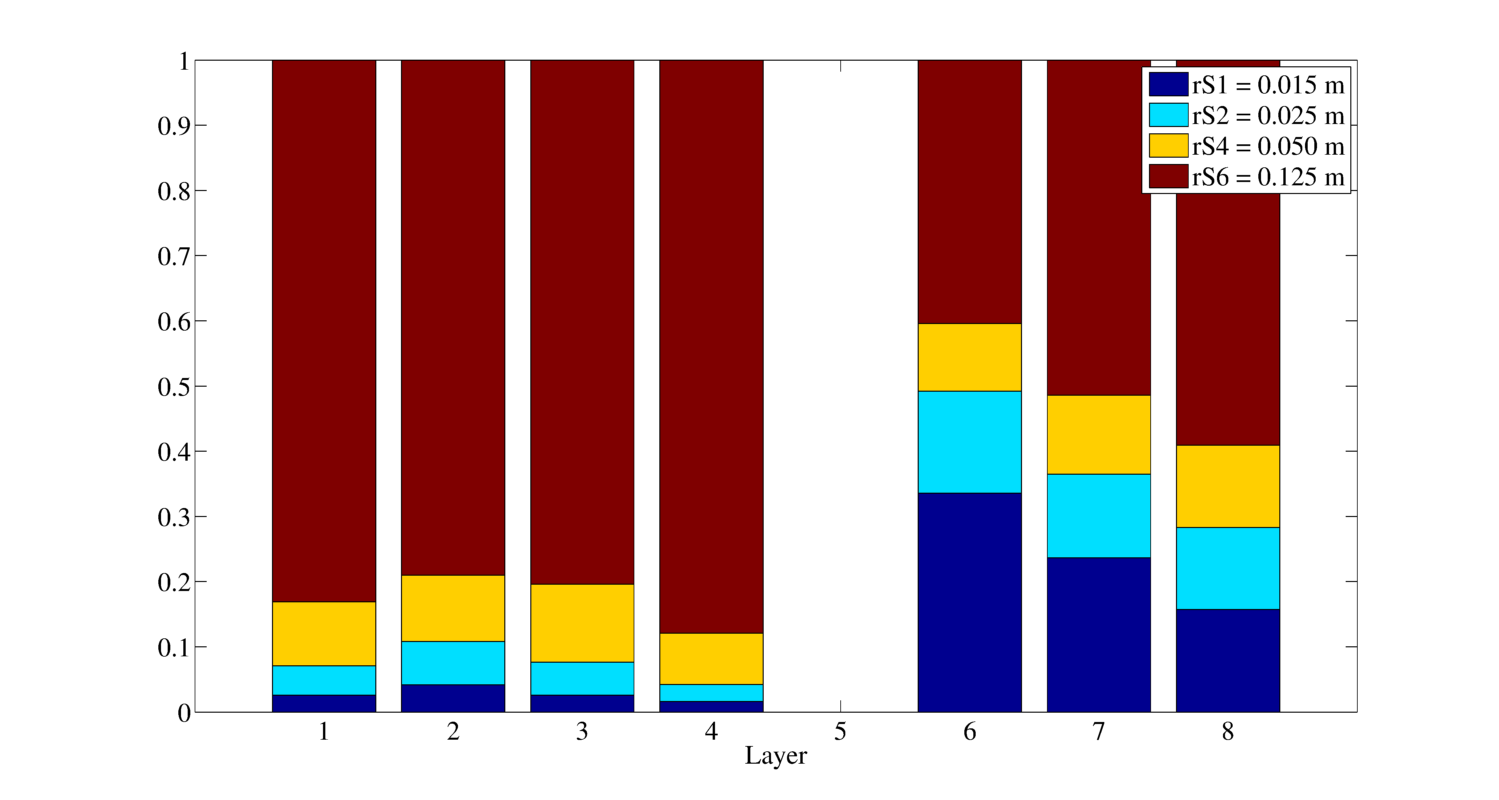
\includegraphics[width=.96\columnwidth]{images/121SinterBarPlot20151111150702}
	  \label{fig:121SinterBarPlot20151111150702}
  }
  \\
    \subfloat[Ratio over the number of the particles of each radius.]
    {
	  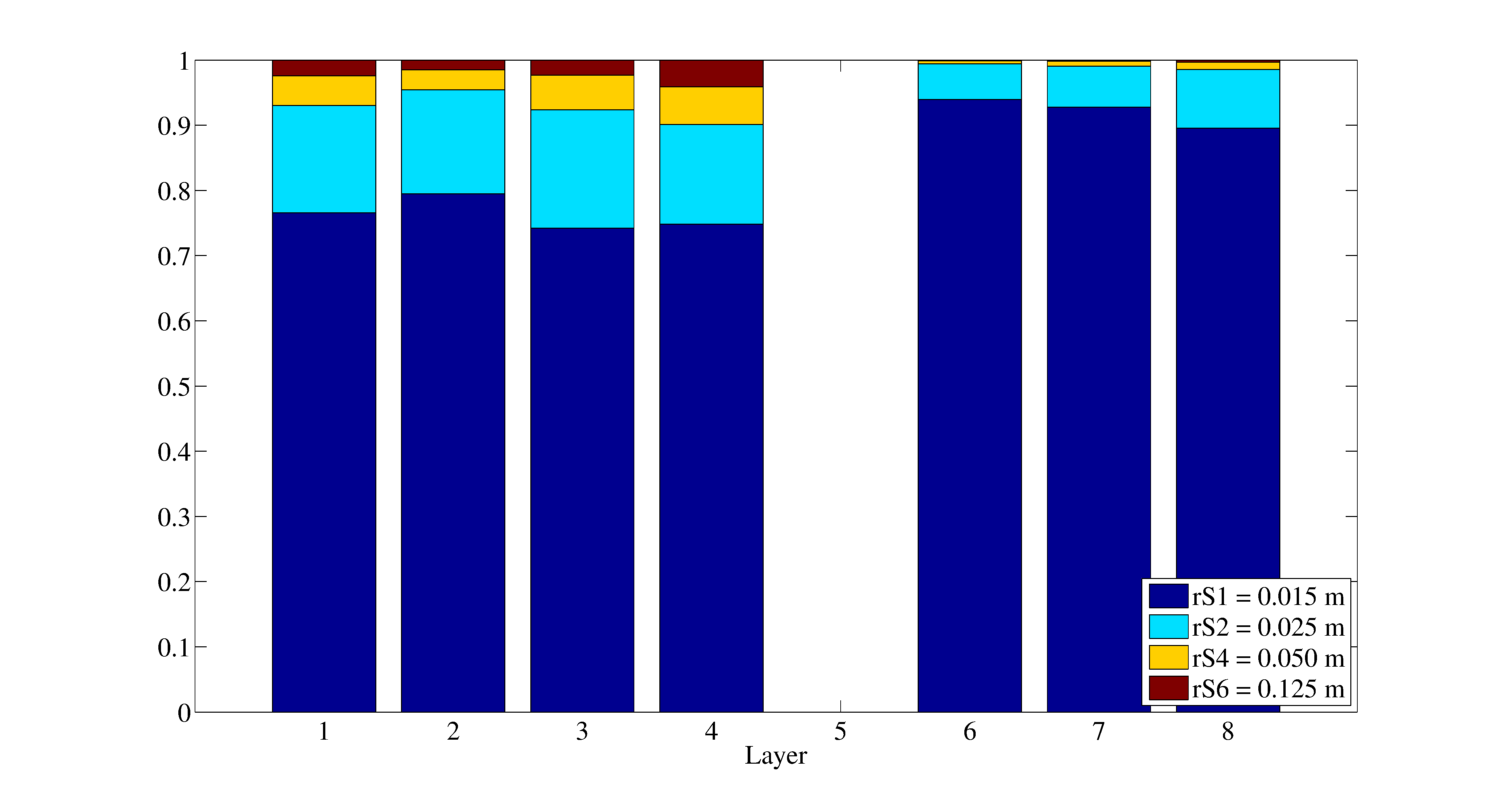
\includegraphics[width=.96\columnwidth]{images/122SinterBarPlot20151123180606}
	  \label{fig:122SinterBarPlot20151123180606}
  }
  \\
  \caption{Sinter bar plot.}
  \label{fig:066sinterbarplot}
\end{figure}
\begin{table}[htbp]
  \centering
  \caption{$DEM$ simulation parameters, particle-particle (p-p) and
  particle-wall (p-w)}
    \begin{tabular}{l|cccccc}
    \hline
          & Young's & coeff. of & coeff. of & sliding & rolling & particles \\
          & modulus & Poisson & restitution & friction &
          friction & density \\
          & [Pa] &  [-] &  [-] &   [-] &  [-] &  $[kg/m^3]$  \\
          \hline
    p-p & 3.00E+08 & 0.4   & 0.2   & 0.91  & 0.35  & 2284 \\
    p-w & 2.00E+08 & 0.4   & 0.2   & 0.65  & 0.25  & - \\
    \hline
    \end{tabular}%
  \label{tab:parameters}%
\end{table}%


The $DEM$ parameters used in the simulation can be found in Table
\ref{tab:parameters}.
The total volume of the particles with different radii in the three considered
layers, variation with time, can
be seen in Fig. \ref{fig:096sinterplots}.

\begin{sidewaysfigure}[htbp]
\centering 
  \subfloat%[Jenike shear cell tester.]
  {
	  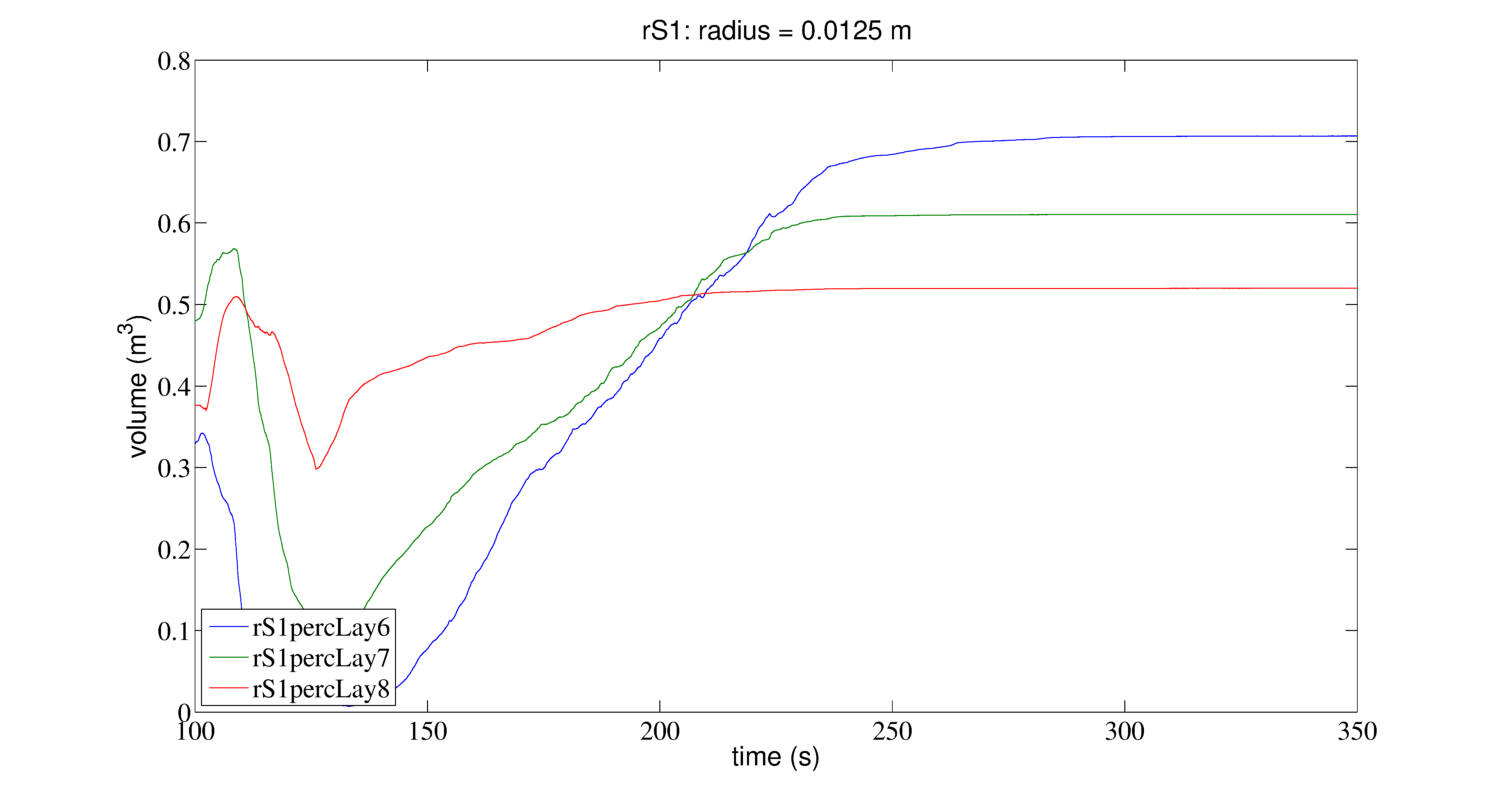
\includegraphics[width=.48\columnwidth]{images/113rS120151111150702}
	  \label{fig:113rS120151111150702}
  }
  \quad
    \subfloat
    %[Simplified Jenike shear cell tester.]
    {
	  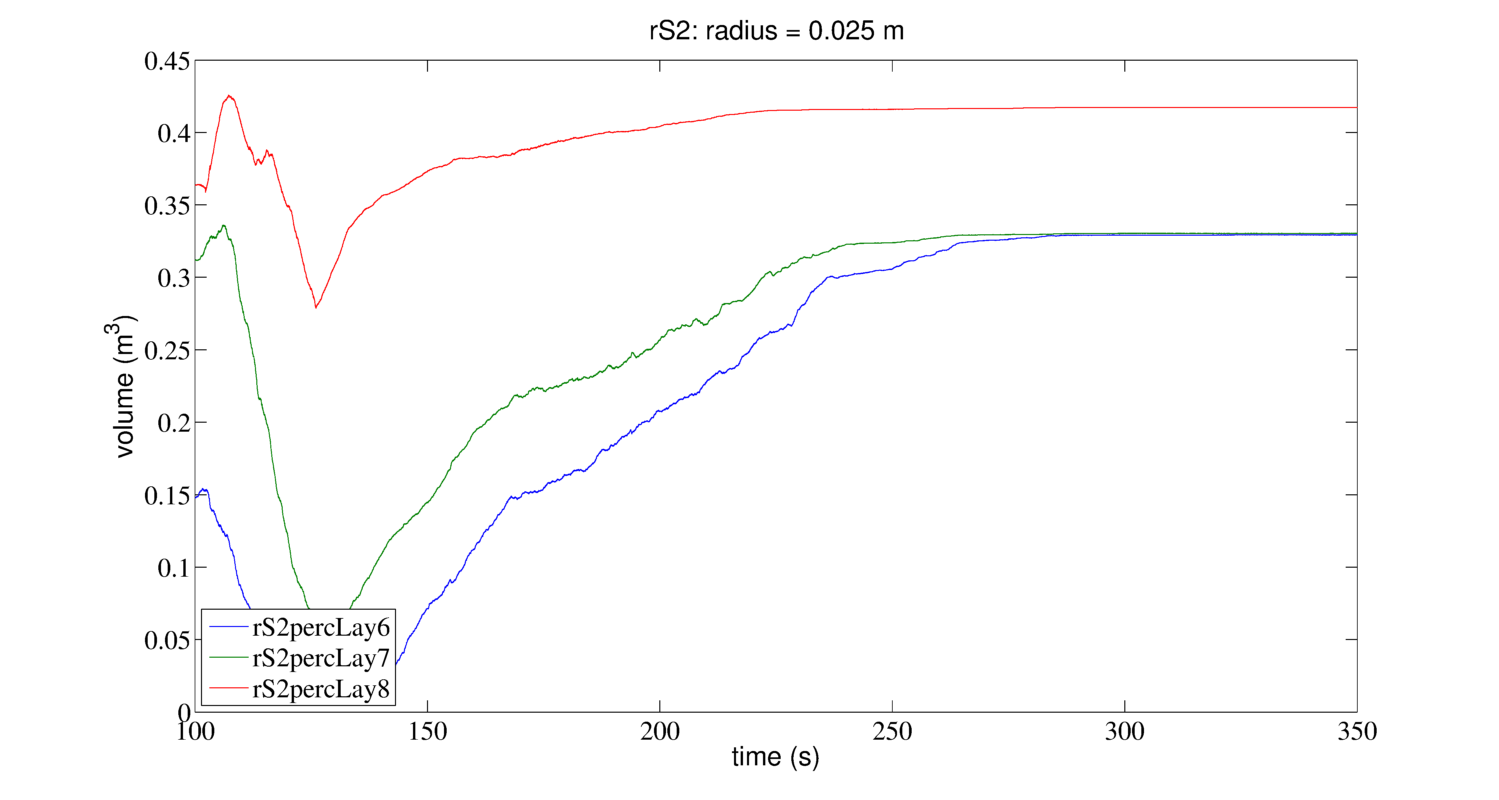
\includegraphics[width=.48\columnwidth]{images/115rS220151111150702}
	  \label{fig:115rS220151111150702}
  }
  \\
  \subfloat%[Jenike shear cell tester layout.]
  {
	  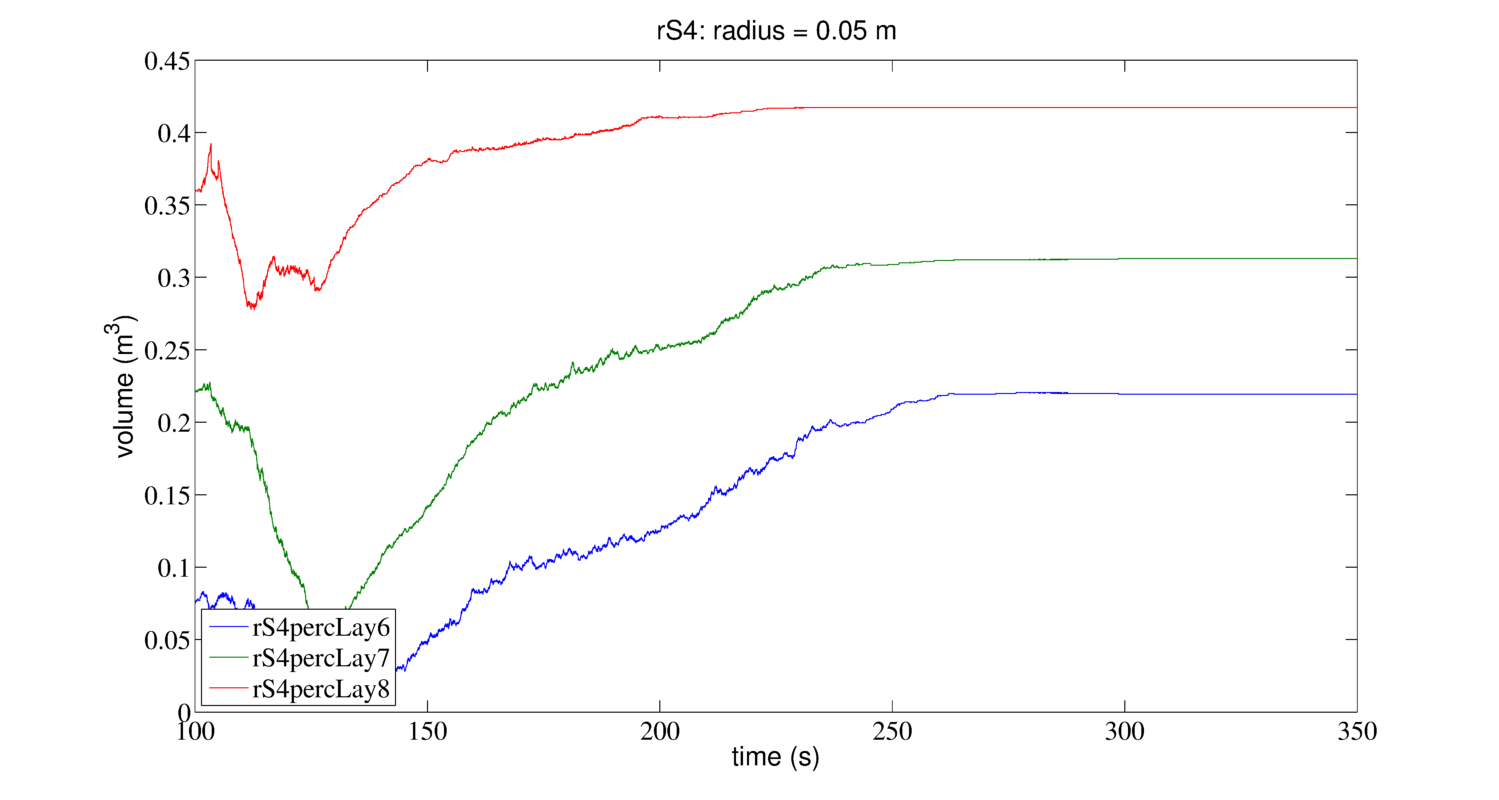
\includegraphics[width=.48\columnwidth]{images/117rS420151111150702}
	  \label{fig:117rS420151111150702}
  }
  \quad
    \subfloat%[Jenike shear cell tester diagram.]
    {
	  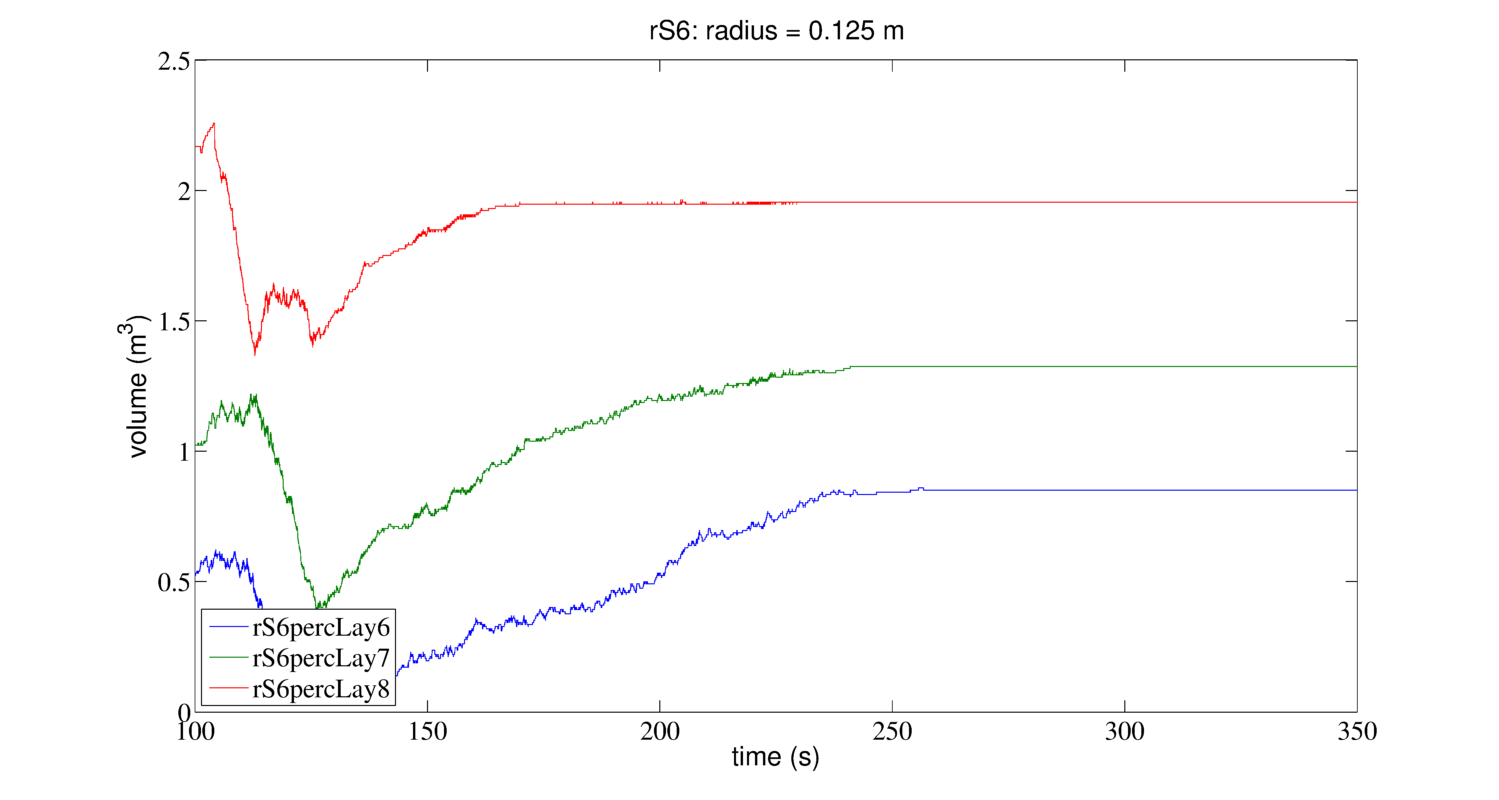
\includegraphics[width=.48\columnwidth]{images/119rS620151111150702}
	  \label{fig:119rS620151111150702}  }
  \\
  \caption{Particle size distribution during the simulation, in $m^3$ of
  material. Once steady state is reached, large particles are more likely in the
  inferior layers, small particles in the superior ones.}
  \label{fig:096sinterplots}
\end{sidewaysfigure}
\begin{figure}[htbp]
\centering 
  \subfloat%[Jenike shear cell tester.]
  {
	  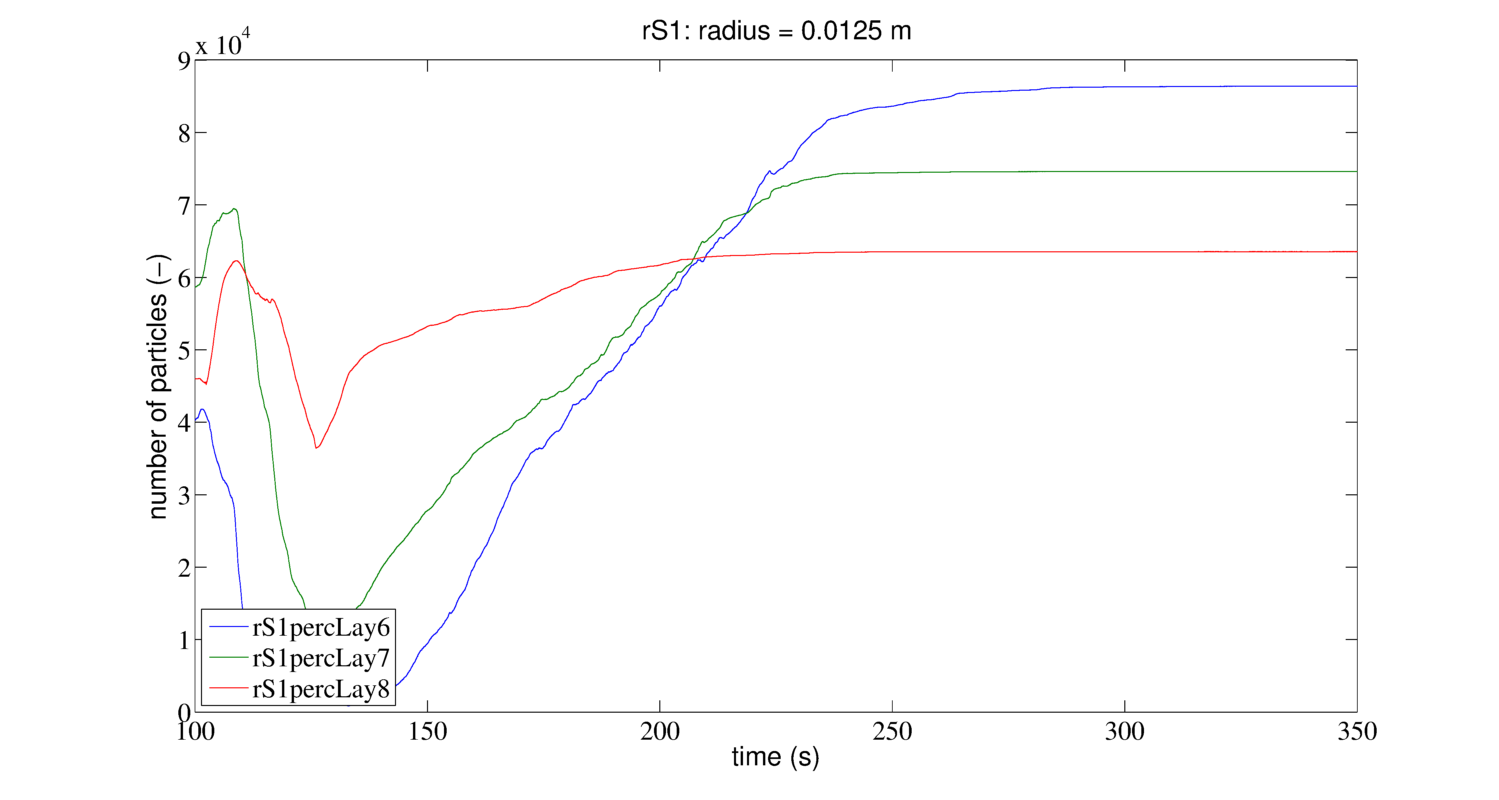
\includegraphics[width=.70\columnwidth]{114rS120151111151255}
	  \label{fig:114rS120151111151255}
  }
  \\
    \subfloat
    %[Simplified Jenike shear cell tester.]
    {
	  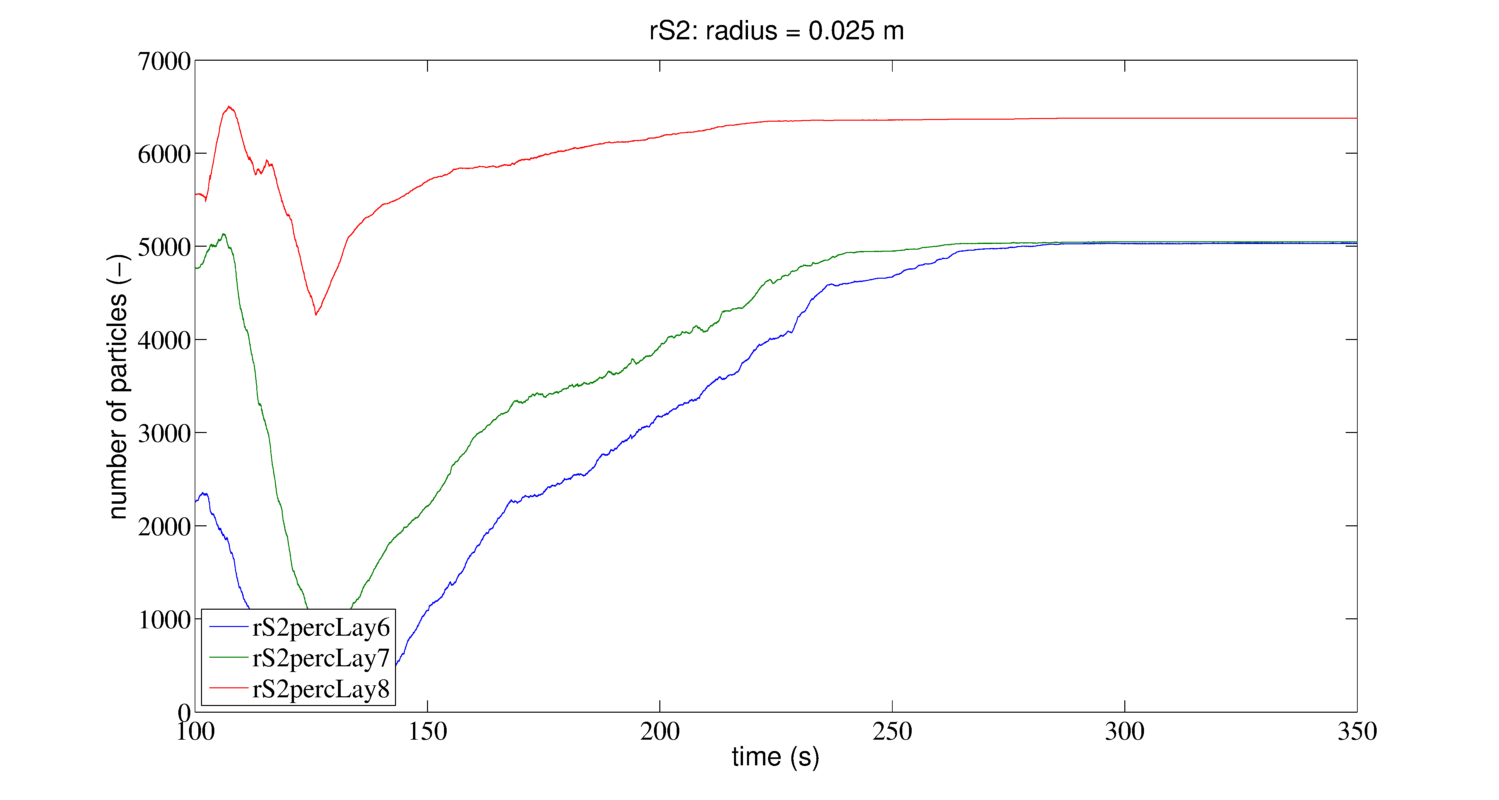
\includegraphics[width=.70\columnwidth]{116rS220151111151255}
	  \label{fig:116rS220151111151255}
  }
  \\
  \subfloat%[Jenike shear cell tester layout.]
  {
	  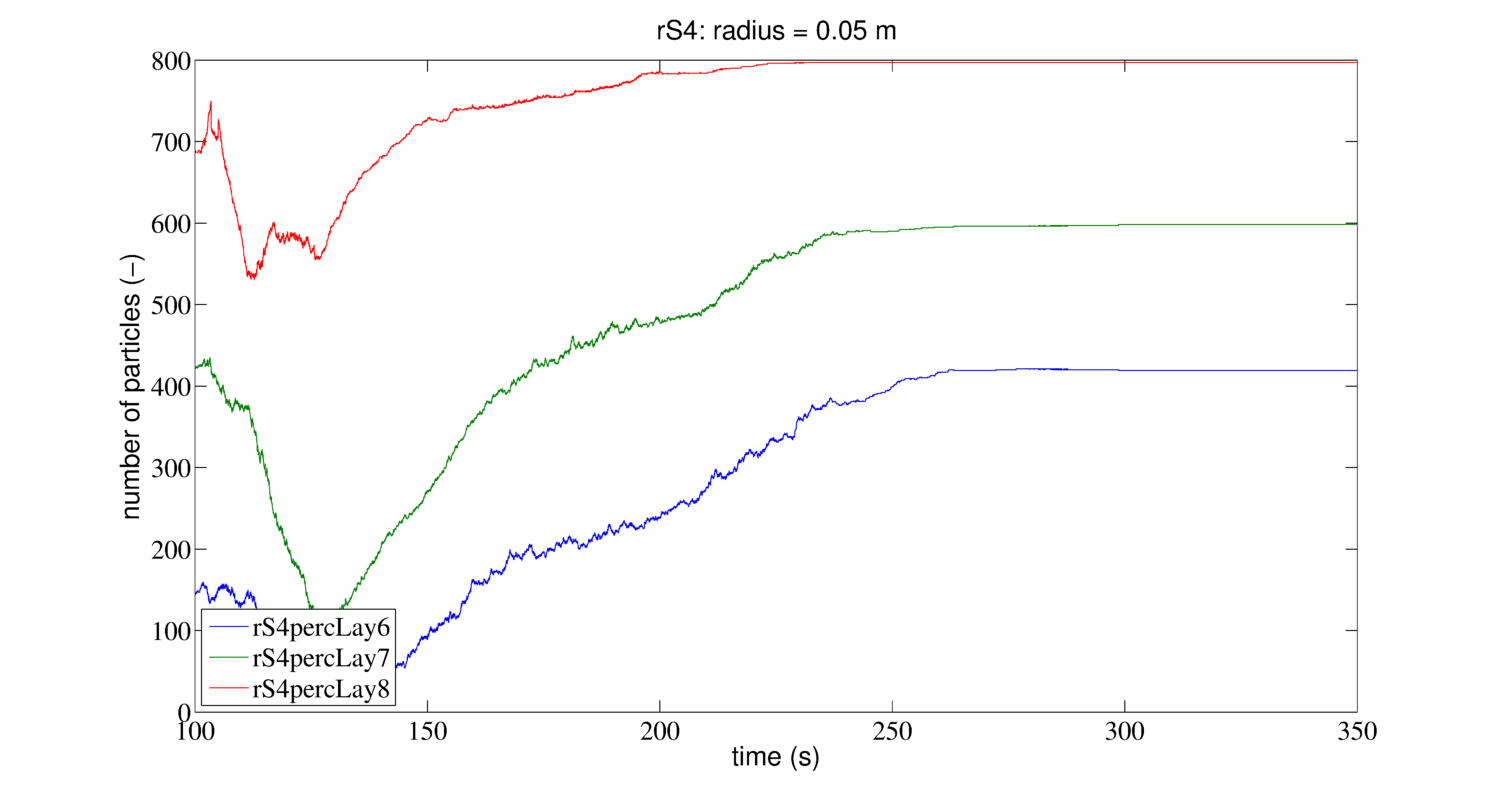
\includegraphics[width=.70\columnwidth]{118rS420151111151255}
	  \label{fig:118rS420151111151255}
  }
  \\
    \subfloat%[Jenike shear cell tester diagram.]
    {
	  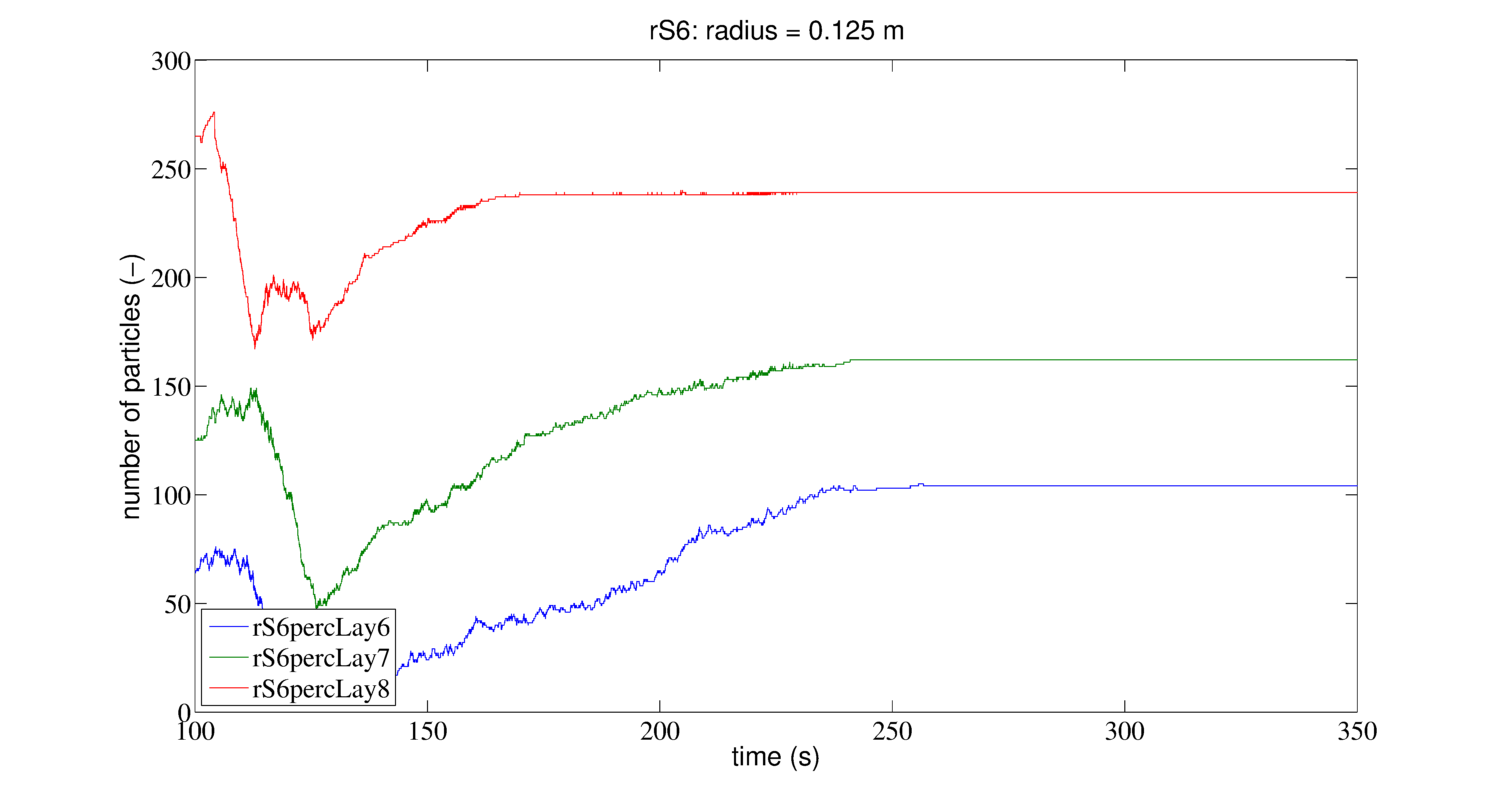
\includegraphics[width=.70\columnwidth]{120rS620151111151255}
	  \label{fig:120rS620151111151255}  }
  \\
  \caption{Particle size distribution during the simulation, number of
  particles.}
  \label{fig:096sinterplots}
\end{figure}


